\section{Der Funktionsbegriff}

\stepcounter{subsection}% Im Original steht vor den Beispielen kein eigener Unterabschnitt (Nummerierung 1.1.1.x)

Der Begriff der \textbf{Funktion} ist in der Mathematik von zentraler Bedeutung. Mit Hilfe von Funktionen werden Zusammenhänge zwischen verschiedenen Objektbereichen beschrieben. Dabei sieht ein Schaubild einer Funktion oft ähnlich aus wie in dem folgenden Bild:

\begin{center}
  \begin{tikzpicture}
    \begin{axis}[width=10cm, height=6.2cm, axis lines=left, xmin=0, xmax=10, ymin=0, ymax=100,
      xtick={0,1,...,10}, ytick={0,10,...,100}, xlabel={$x$}, ylabel={$y$}, samples=100, tick label style={font=\footnotesize}]
      \addplot[thick, black, domain=0:10] {2 + x^2};
    \end{axis}
  \end{tikzpicture}
\end{center}

Dies ist selbstverständlich eine starke Abstraktion: Hinter dem Beispiel mag hier etwa der Zusammenhang zwischen einer Produktionsmenge in Tausend Stück ($x$-Achse) und den dabei anfallenden Produktionskosten in Tausend Euro ($y$-Achse) stehen.

Die folgenden Beispiele verdeutlichen die Bedeutung des Funktionsbegriffs in unterschiedlichen Anwendungskontexten.
\begin{itemize}
  \item Die zu entrichtende Einkommensteuer hängt (bei gegebenen Bedingungen wie Steuerklasse, Kinderzahl usw.) in eindeutiger Weise vom erzielten Einkommen ab. Die Einkommensteuer ist eine Funktion des Einkommens.
  \item Die in einem Unternehmen anfallenden Produktionskosten hängen in eindeutiger Weise von der produzierten Menge ab: Wird mehr produziert, so fallen dafür mehr Kosten an. (Können die Produkte alle verkauft werden, wird dadurch u.\,U. ein höherer Gewinn erzielt.) Die Produktionskosten sind eine Funktion der produzierten Menge (der Gewinn übrigens auch, aber eine andere).
  \item Zieht man ein gespanntes Gummiband auseinander, so wird es länger -- je mehr man zieht, desto länger wird es (jedenfalls bis zu einer gewissen Länge, ab der es nicht mehr weiter gedehnt werden kann bzw. sogar reißt). Die Länge des Bandes ist eine Funktion der beim Ziehen aufgewendeten Kraft.
  \item Frau K. kauft an jedem Morgen in der Bäckerei nebenan einige Brötchen, das Stück zu 23 Cent. Die Anzahl gekaufter Brötchen ist nicht immer gleich, weil manchmal Gäste zum Frühstück kommen. Der für die Brötchen zu zahlende Betrag ergibt sich in eindeutiger Weise aus der Brötchenanzahl, man sagt: Der Preis ist eine Funktion der Anzahl gekaufter Brötchen (1 Brötchen 23 Cent, 2 Brötchen 46 Cent etc.)
\end{itemize}

Bei den obigen Beispielen sind alle betrachteten Größen durch Zahlen beschreibbar (Brötchenanzahl, Preis, Länge des Gummibandes, Einkommen etc.). Der Funktionsbegriff ist jedoch wesentlich allgemeiner angelegt -- er lässt auch die Zuordnung zwischen andersartigen Objekten zu. Hierzu ein Beispiel:
\begin{itemize}
  \item Jedem in Deutschland zugelassenen Auto ist in eindeutiger Weise ein Autokennzeichen zugeordnet. Das Autokennzeichen ist eine Funktion des einzelnen betrachteten Autos.
\end{itemize}

Mit der Formulierung »in eindeutiger Weise«, die in den Beispielen verwendet wird, ist gemeint, dass (am Brötchenbeispiel) durch die Größe »Brötchenanzahl« die Größe »zu zahlender Preis« eindeutig festgelegt ist, man kann ihn daraus \emph{berechnen}. Der allgemeine Begriff der Funktion beinhaltet allerdings nur die eindeutige Festlegung der einen Größe durch die andere, auf die Berechenbarkeit wird notfalls verzichtet -- so etwa beim Autokennzeichen. Dadurch fällt z.\,B. auch \emph{die Anzahl der Kopfhaare bei jedem der am 31.12.2020 auf der Erde lebenden Menschen} unter den Begriff der Funktion, obwohl man die Funktionswerte hier sicher nicht ausrechnen kann.

Man kann dies alles auch in der Sprache der Mengenlehre sagen: Jedem Element $x$ einer Menge $D$ wird durch eine Zuordnungsvorschrift $f$ ein durch das Element $x$ eindeutig bestimmtes Element $y = f(x)$ einer Menge $B$ zugeordnet. Die Menge $D$ wird dabei als \textbf{Definitionsbereich} und die Menge $B$ als \textbf{Bildbereich} von $f$ bezeichnet.

\merkbox{Funktionen, deren Definitions- und Bildbereiche aus reellen Zahlen bestehen, für die also $D \subseteq \mathbb{R}$ und $B \subseteq \mathbb{R}$ gilt, heißen \textbf{reellwertige Funktionen einer reellen Veränderlichen} oder kurz \textbf{reelle Funktionen}.}

\textbf{Hinweis:} Der Bildbereich $B$ wird in der Literatur gelegentlich auch als \textbf{Wertebereich} $W$ oder als \textbf{Wertevorrat} $W_f$ der Funktion $f$ bezeichnet.

Statt $y = f(x)$ schreibt man auch $x \rightarrow y$ (gelesen: $x$ wird $y$ zugeordnet) oder $x \rightarrow f(x)$ (gelesen: $x$ wird $f$ von $x$ zugeordnet). $x \rightarrow y$ oder $x \rightarrow f(x)$ wird dabei als \textbf{Abbildungs-} oder \textbf{Zuordnungsvorschrift} bezeichnet.

Variiert $x$ im Definitionsbereich $D$ von $f$, so wird $x$ als \textbf{unabhängige Veränderliche} oder \textbf{unabhängige Variable} oder kurz als \textbf{Argument} bezeichnet. Variiert $y = f(x)$ im Bildbereich $B$, so wird $y$ als \textbf{abhängige Veränderliche} oder als \textbf{Funktionswert} bezeichnet.

Zur exakten Beschreibung einer Funktion $f$ gehört somit zweierlei:
\begin{itemize}
  \item die Festlegung des Definitions- und Bildbereiches
  \item die Angabe der eigentlichen Zuordnungsvorschrift
\end{itemize}

Die Abbildungs- oder Zuordnungsvorschrift $x \rightarrow y$ oder $x \rightarrow f(x)$ kann in unterschiedlicher Weise angegeben werden, was zu verschiedenen Funktionsdarstellungen führt -- dies wird im nächsten Abschnitt genauer beleuchtet. Dabei werden nur noch Funktionen betrachtet, die durch Zahlen (bzw. sogar durch eine Formel) beschrieben werden können. Solche reellen Funktionen sind für die unmittelbare Anwendung am wichtigsten und werden üblicherweise auch in der Schulmathematik behandelt.

Die Themen \textbf{Wichtige Funktionen}, \textbf{Differenzialrechnung zur Extremwertbestimmung} und \textbf{Kurvendiskussion} werden anschließend behandelt.

\subsubsection{Übungsaufgabe}

\begin{graukasten}
  Jedem Menschen kann seine Mutter zugeordnet werden -- bildet diese Zuordnung eine Funktion? Wie ist es umgekehrt, wenn jeder Mutter eines ihrer Kinder zugeordnet wird?
\end{graukasten}

\section{Darstellung von Funktionen}

Es geht in diesem Abschnitt um die Frage, wie man eine reelle Funktion beschreiben kann, d.\,h. wie man präzise ausdrücken kann, über welche Funktion man redet. Fast immer wird dazu eine der drei folgenden Möglichkeiten verwendet:
\begin{itemize}
  \item tabellarische Darstellung (\textbf{Tabelle})
  \item analytische Darstellung (\textbf{Funktionsgleichung})
  \item grafische Darstellung (in einem \textbf{Koordinatensystem})
\end{itemize}

Dies wird jetzt an Beispielen aufgezeigt.

\subsection{Beispiel Brötchenpreise}

\textbf{Tabelle:}
\begin{center}
  \begin{tabular}{rr}
    \hline
    Brötchen & Cent\\
    \hline
    1 & 23\\
    2 & 46\\
    3 & 69\\
    $\ldots$ & $\ldots$\\
    \hline
  \end{tabular}
\end{center}

\textbf{Funktionsgleichung:} $y = 23 \cdot x$

\textbf{Grafische Darstellung:}
\begin{center}
  \begin{tikzpicture}
    \begin{axis}[width=9cm, height=6cm, axis lines=left, xmin=0, xmax=6.5, ymin=0, ymax=145,
      xtick={0,1,...,6}, ytick={0,20,...,140}, xlabel={$x$}, ylabel={$y$}, tick label style={font=\footnotesize}]
      \addplot[blue, thick, domain=0:6] {23*x};
    \end{axis}
  \end{tikzpicture}
\end{center}
\beispielende

\subsection{Beispiel Einkommensteuer 2020 nach §\,32a EStG}

\textbf{Tabelle (Auszug):}
\begin{center}
  \begin{tabular}{rr}
    \hline
    Einkommen & Steuer\\
    \hline
    $\ldots$ & $\ldots$\\
    33500 & 6282\\
    34000 & 6442\\
    34500 & 6604\\
    35000 & 6767\\
    35500 & 6930\\
    $\ldots$ & $\ldots$\\
    \hline
  \end{tabular}
\end{center}

\textbf{Funktionsgleichung:}

\begin{center}
\resizebox{0.95\linewidth}{!}{$
f(x) = \begin{cases}
  0 & \text{falls } x \leq 9408\\
  \left(972{,}87 \cdot \dfrac{x - 9408}{10000} + 1400\right) \cdot \dfrac{x - 9408}{10000} & \text{falls } 9408 \leq x \leq 14532\\
  \left(212{,}02 \cdot \dfrac{x - 14532}{10000} + 2397\right) \cdot \dfrac{x - 14532}{10000} + 972{,}79 & \text{falls } 14533 \leq x \leq 57051\\
  0{,}42 \cdot x - 8963{,}74 & \text{falls } 57052 \leq x \leq 270500\\
  0{,}45 \cdot x - 17078{,}74 & \text{falls } 270500 \leq x
\end{cases}
$}
\end{center}
(Dabei wird das Ergebnis zum Schluss noch auf den vollen Euro-Betrag abgerundet.)

\textbf{Grafische Darstellung:}
\begin{center}
  \begin{tikzpicture}
    \begin{axis}[width=10cm, height=7cm, axis lines=left, xmin=0, xmax=300000, ymin=0, ymax=120000,
      xtick={0,50000,...,300000}, ytick={0,20000,...,120000}, xticklabel style={rotate=45, anchor=east, font=\tiny},
      yticklabel style={font=\tiny}, xlabel={$x$}, ylabel={$y$}, scaled x ticks=false, scaled y ticks=false,
      xticklabels={0,50.000,100.000,150.000,200.000,250.000,300.000}, yticklabels={0,20.000,40.000,60.000,80.000,100.000,120.000}, samples=200]
      \addplot[domain=9408:14532, teal, thick] {(972.87*(x-9408)/10000+1400)*(x-9408)/10000};
      \addplot[domain=14532:57051, orange, thick] {(212.02*(x-14532)/10000+2397)*(x-14532)/10000+972.79};
      \addplot[domain=57051:270500, orange, thick] {0.42*x-8963.74};
      \addplot[domain=270500:300000, purple, thick] {0.45*x-17078.74};
    \end{axis}
  \end{tikzpicture}
\end{center}
\beispielende

\subsection{Beispiel Weg-Zeit-Funktion eines fallenden Apfels}

Eine \textbf{Tabelle} ist in diesem Fall nicht sinnvoll.

\textbf{Funktionsgleichung:} $s = 4{,}9 \cdot t^2$

\textbf{Grafische Darstellung:}
\begin{center}
  \begin{tikzpicture}
    \begin{axis}[width=9cm, height=6cm, axis lines=left, xmin=0, xmax=5.3, ymin=0, ymax=130,
      xtick={0,1,...,5}, ytick={0,20,...,120}, xlabel={$t$ [sec]}, ylabel={$s$ [m]}, tick label style={font=\footnotesize}]
      \addplot[blue, thick, domain=0:5] {4.9*x^2};
    \end{axis}
  \end{tikzpicture}
\end{center}
\beispielende

Jedes dieser drei Beispiele hat seine Eigenheiten.

Beim \textbf{Beispiel Brötchenpreise} ist bemerkenswert, dass in der Tabelle nur ganze Brötchen aufgeführt sind (und z.\,B. nicht $\tfrac{3}{2}$ oder 1{,}4 Brötchen), man jedoch bei der Funktionsgleichung und der grafischen Darstellung diese Beschränkung fallen lässt. Die mathematische Beschreibung geht so über die Bedeutung im realen Beispiel hinaus. Dies ist durchaus nicht ungewöhnlich, die mathematische Beschreibung wird so bequemer. Man \emph{könnte} es allerdings auch anders machen -- bei der Einschränkung auf ganze Zahlen ergäbe sich die folgende Grafik:

\begin{center}
  \begin{tikzpicture}
    \begin{axis}[width=9cm, height=6cm, axis lines=left, xmin=0, xmax=5.3, ymin=0, ymax=120,
      xtick={0,1,...,5}, ytick={0,20,...,100}, xlabel={$x$}, tick label style={font=\footnotesize}]
      \addplot[only marks, mark=*, mark size=1.5pt, blue!50!black] coordinates {(0,0) (1,23) (2,46) (3,69) (4,92) (5,115)};
    \end{axis}
  \end{tikzpicture}
\end{center}

Beim \textbf{Beispiel Einkommensteuer} wird die Beschränkung einer Beschreibung mit einer Tabelle deutlich: Als Einkommen sind nur Vielfache von 500\,€ eingetragen, sonst würde die Tabelle zu umfangreich. Dagegen sind die Beschreibungen durch Funktionsgleichung und Grafik detaillierter. (Allerdings ist der Einfachheit halber die Funktion hier »verstetigt«. In Wirklichkeit werden die Beträge von Einkommen wie zu entrichtender Steuer jeweils auf einen vollen Euro-Betrag abgerundet.)

An der Grafik ist nur schlecht zu erkennen, dass zwei Teile der »aneinander gestückelten« Kurve Parabelstücke sind, die anderen sind Geradenstücke. (Zum Begriff der \textbf{Parabel} mehr im nächsten Abschnitt.) An dem folgenden Ausschnitt, der nur die ersten drei Stücke zeigt, ist dies besser zu sehen:

\begin{center}
  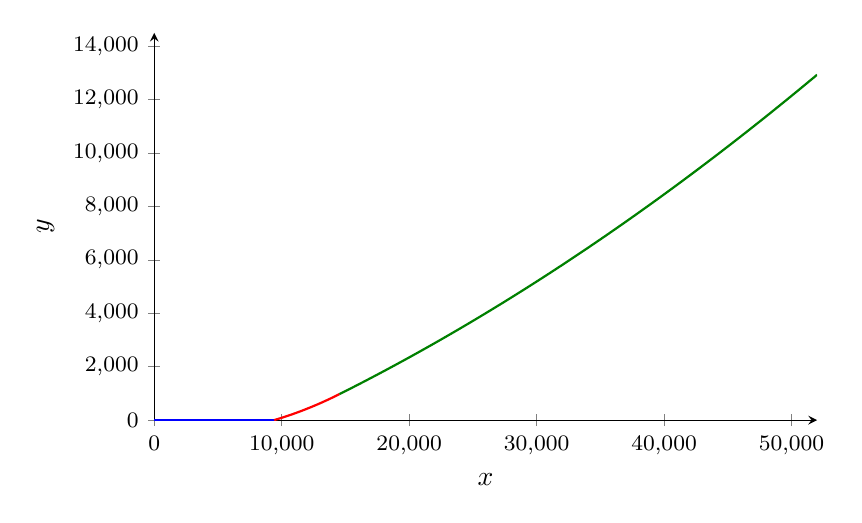
\begin{tikzpicture}
    \begin{axis}[width=10cm, height=6.5cm, axis lines=left, xmin=0, xmax=52000, ymin=0, ymax=14500,
      xtick={0,10000,...,50000}, ytick={0,2000,...,14000}, xlabel={$x$}, ylabel={$y$}, scaled x ticks=false, scaled y ticks=false, tick label style={font=\footnotesize}, samples=200]
      \addplot[domain=0:9408, blue, thick] {0};
      \addplot[domain=9408:14532, red, thick] {(972.87*(x-9408)/10000+1400)*(x-9408)/10000};
      \addplot[domain=14532:52000, green!50!black, thick] {(212.02*(x-14532)/10000+2397)*(x-14532)/10000+972.79};
    \end{axis}
  \end{tikzpicture}
\end{center}

Das \textbf{Apfelbeispiel} ist Teil des klassischen Physikunterrichts in der Schule. Auch hier sieht man an dem $t^2$ in der Formel, dass sich eine Parabel ergibt. (Anders gesagt: In der doppelten Zeit fällt der Apfel vier Mal so tief.) Da hier auch Bruchteile von Sekunden von Interesse sind, leuchtet es ein, dass die Beschreibung der Funktion durch eine Tabelle nicht sinnvoll wäre.

Generell lässt sich eine Funktion nur mit der analytischen Darstellung präzise und unmissverständlich beschreiben -- eine Tabelle ist in der Regel lückenhaft, die grafische Darstellung ungenau. Trotzdem kann besonders die grafische Darstellung eine große Hilfe sein, sich einen Eindruck von einer Funktion zu verschaffen.

\subsubsection{Übungsaufgabe}

\begin{graukasten}
  In einer Kleingartensiedlung werden rechteckige Grundstücke mit jeweils 1000\,qm angeboten. Es werden Grundstücke mit 25\,m Länge und 40\,m Tiefe angeboten, andere sind 32\,m lang und 31{,}25\,m tief. Stellen Sie die Tiefe als Funktion der Länge dar, wenn die Länge zwischen 20 und 50\,m variiert; zeichnen Sie ein Schaubild der Funktion.
\end{graukasten}

\section{Einige weitere Beispiele}

Anhand einiger weiterer Beispiele soll die Bedeutung des Funktionsbegriffs noch einmal herausgestellt werden. Es geht auch um die Frage: Warum \emph{möchte} man überhaupt Funktionen exakt beschreiben?

\stepcounter{subsection}% Im Original steht vor den Beispielen kein eigener Unterabschnitt (Nummerierung 1.3.1.x)

\subsubsection{Beispiel}

Für die Produktion der Papierfassung von Lerneinheit 3 zu »Wirtschaftsmathematik« haben sich Gesamtkosten herausgestellt als
\[ K(x) = 2x + 1000 , \]
wobei $x$ die Anzahl der gedruckten Exemplare bezeichnet. Dies bedeutet: Werden $x = 10$ Exemplare hergestellt, so kostet dies
\[ K(10) = 2 \cdot 10 + 1000 = 1020\,€ , \]
die Herstellung von $x = 100$ Exemplaren schlägt mit
\[ K(100) = 2 \cdot 100 + 1000 = 1200\,€ \]
zu Buche.\beispielende

Die Funktion in dem Beispiel wird beschrieben durch eine \textbf{Funktionsgleichung} der Form
\[ K(x) = \ldots , \]
wo rechts ein mathematischer Ausdruck steht, der von der \textbf{Veränderlichen} (bzw. \textbf{Variablen}) $x$ abhängt, die in dem Beispiel die Anzahl der gedruckten Lerneinheiten darstellt.

Die Beschreibung durch eine Funktionsgleichung ist der »Idealfall«, denn davon ausgehend kann man Eigenschaften der Funktion mit rein mathematischen Methoden untersuchen.

Kommen wir im nächsten Schritt zu der eingangs gestellten Frage: Warum \emph{möchte} man überhaupt Funktionen beschreiben? Das Beispiel legt eine Antwort nahe: Wenn die Gesamtkosten sich tatsächlich so verhalten, wie die Funktionsgleichung besagt, so kann man nun auch Kosten \emph{voraussagen} -- man weiß z.\,B., mit welchen Kosten man bei der Produktion von 200 Lerneinheiten zu rechnen hat!

An dem Beispiel ist ferner die Beobachtung interessant, dass auch Kosten anfallen, wenn \emph{keine} Lerneinheiten produziert werden -- dies ist typisch für Kostenfunktionen:
\[ K(0) = 2 \cdot 0 + 1000 = 1000\,€ . \]
Man spricht von den \textbf{Fixkosten} $K_f$ und kann nun auch schreiben:
\[ K(x) = 2 \cdot x + K_f \]
Den Summanden $2 \cdot x$ nennt man die \textbf{variablen Kosten}. Allgemein ist eine Kostenfunktion als Summe
\[ K(x) = V(x) + K_f \]
darstellbar, wobei $V(x)$ für die von $x$ abhängigen variablen Kosten steht und $K_f$ für die Fixkosten.

\subsubsection{Beispiel}

Kostenfunktionen $K(x)$, mit denen man die Gesamtkosten (in irgendwelchen Geldeinheiten, es müssen keine Euro sein) für die Herstellung von $x$ Einheiten eines Gutes in einem Unternehmen beschreibt, haben oft die folgenden Eigenschaften:
\begin{itemize}
  \item Die Fixkosten sind positiv, d.\,h. $K(0) = K_f > 0$.
  \item Wenn $x$ größer wird, steigen auch die Kosten.
  \item Zu Beginn steigen die Kosten schnell, aber die Kostensteigerung verlangsamt sich dann, weil die Fertigungseinrichtungen des Unternehmens (z.\,B. Maschinen) besser genutzt werden.
  \item Ab einer gewissen Größe von $x$ steigen die Kosten wieder schneller, z.\,B. wegen technischer Engpässe oder weil neues Personal eingestellt werden muss.
\end{itemize}

Mit wirtschaftswissenschaftlichen Argumenten lässt sich zeigen, dass Funktionen der Form
\[ K(x) = a x^3 + b x^2 + c x + d \]
sich für die Beschreibung solcher Kostenfunktionen gut eignen, wenn man für die Konstanten $a$, $b$, $c$ und $d$ voraussetzt:
\[ a > 0, \quad b < 0, \quad c > 0, \quad d > 0, \quad 3ac > b^2 \]
Man spricht hier von einer \textbf{ertragsgesetzlichen Kostenfunktion}. Ein Beispiel ist
\[ K(x) = 0{,}02 x^3 - 2 x^2 + 80 x + 12000 \]
(überprüfen Sie, dass die Bedingungen alle erfüllt sind!)

Im Schaubild sieht die Funktion folgendermaßen aus. Beachten Sie auch die unterschiedliche Wahl der Skalen auf den beiden Achsen!

\begin{center}
  \begin{tikzpicture}
    \begin{axis}[width=10cm, height=7cm, axis lines=left, xmin=0, xmax=85, ymin=12000, ymax=16000,
      xtick={0,10,...,80}, ytick={12000,13000,...,16000}, xlabel={$x$}, ylabel={$K(x)$}, tick label style={font=\footnotesize}, samples=100]
      \addplot[thick, black, domain=0:80] {0.02*x^3-2*x^2+80*x+12000};
    \end{axis}
  \end{tikzpicture}
\end{center}
\beispielende

Wie genau man zu einer Kostenfunktionsgleichung wie im letzten Beispiel kommt, fällt nicht in die Zuständigkeit einer Mathematik-Veranstaltung -- dafür sind die Wirtschaftswissenschaftler zuständig. In den folgenden Kapiteln der vorliegenden Mathematik-Lerneinheit werden Ihnen oft Funktionen bzw. Funktionsgleichungen begegnen, die als abstrakte mathematische Objekte betrachtet werden, d.\,h. bei denen überhaupt nicht darüber gesprochen wird, ob sie einen ökonomischen, technischen oder anderen Zusammenhang beschreiben. Diese Vorgehensweise der Mathematik ist allerdings nicht ungewöhnlich: Wenn wir sagen »Zwei plus Zwei ergibt Vier«, so muss auch nicht darüber geredet werden, ob es um Äpfel, Autos oder Gedanken geht! Wenn wir also von der Funktion
\[ f(x) = 2x^2 - x + 8 \]
sprechen, so muss nicht klar sein, welches reale Phänomen man damit zu beschreiben versucht. Trotzdem werden wir selbstverständlich oft Beispiele aus dem Bereich der Ökonomie heranziehen.

\subsubsection{Beispiel}

Die Funktionsgleichung $y = f(x) = 2x + 1$ sei gegeben. Für jeden $x$-Wert ergibt sich durch Einsetzen in die Funktionsgleichung der zugehörige $y$-Wert. Die folgende Abbildung zeigt das zugehörige Schaubild der Funktion.

\begin{center}
  \begin{tikzpicture}
    \begin{axis}[width=9cm, height=6.5cm, axis lines=middle, xmin=-4.5, xmax=4.6, ymin=-7, ymax=9.5,
      xtick={-4,...,4}, ytick={-6,-4,...,8}, xlabel={$x$}, ylabel={$y$}, tick label style={font=\footnotesize}]
      \addplot[black, thick, domain=-4.4:4.2] {2*x+1};
    \end{axis}
  \end{tikzpicture}
\end{center}

Wie allgemein üblich, wird im Folgenden nicht immer scharf zwischen Funktion und Funktionsgleichung unterschieden, d.\,h. wir werden etwa von der »Funktion $y = f(x)$« sprechen.\beispielende

\subsubsection{Beispiel}

Wir betrachten die Funktion $y = \dfrac{2}{x - 3}$. Ein Schaubild sieht folgendermaßen aus:

\begin{center}
  \begin{tikzpicture}
    \begin{axis}[width=9cm, height=8cm, axis lines=middle, xmin=-5.2, xmax=5.3, ymin=-6.5, ymax=5.5,
      xtick={-5,...,5}, ytick={-6,...,5}, xlabel={$x$}, ylabel={$y$}, tick label style={font=\footnotesize}, samples=300]
      \addplot[black, thick, domain=-5.2:2.85] {2/(x-3)};
      \addplot[black, thick, domain=3.15:5.3] {2/(x-3)};
      \addplot[dashed, gray] coordinates {(3,-6.5) (3,5.5)};
    \end{axis}
  \end{tikzpicture}
\end{center}

Offenbar darf man für $x$ nicht den Wert 3 einsetzen, denn durch Null darf nicht dividiert werden! Im Schaubild ist dementsprechend zu sehen, dass $x = 3$ nicht zugelassen ist (an der gestrichelten senkrechten Linie zu erkennen).\beispielende

Ist eine Funktion durch eine Funktionsgleichung gegeben, ohne dass über den Anwendungskontext gesprochen wird, so geht man auf Seiten der Mathematik immer davon aus, dass der größtmögliche Definitionsbereich angenommen wird. In Beispiel 1.3.1.3 nimmt man als Definitionsbereich konsequenterweise die Menge \emph{aller} reellen Zahlen, in Beispiel 1.3.1.4 muss man nur $x = 3$ ausnehmen. Ist demgegenüber der Anwendungskontext bekannt, so ist oft nur ein eingeschränkter Definitionsbereich von Interesse -- beispielsweise bei einer Kostenfunktion $K(x)$ nur Werte $x \geq 0$.

\subsubsection{Übungsaufgabe}

\begin{graukasten}
  Welche der folgenden Zuordnungen sind Funktionen?
  \begin{enumerate}[label=\alph*)]
    \item Schüler $\rightarrow$ Schulklasse
    \item Kfz $\rightarrow$ Anzahl der Räder
    \item $x \rightarrow 2x^2 + 1$
    \item $x \rightarrow \pm\sqrt{x}$
    \item $x \rightarrow \sqrt{x}$
  \end{enumerate}
\end{graukasten}
